\section{Influenza Virus Structure}

\begin{table}[h!]
\centering
\caption{vRNP segments of influenza virus}
\label{table:fluSegments}

\begin{tabular}{p{2cm} p{11cm}}
\hline 
\textbf{Segment}&    \textbf{Protein}\\
\hline
PB2&    polymerase subunit PB2\\
\hline
PB1&    \tabitem polymerase subunit PB1\\
   &    \tabitem protein PB1-F2, which has apoptotic function\\
   &    \tabitem protein PB1-N40 \cite{dubois2014influenza}\\
\hline
PA&     \tabitem polymerase subunit PA\\
  &     \tabitem protein PA-X, which regulates host translation shutoff \cite{khaperskyy2016selective}\\
  &     \tabitem protein PA-N155 \cite{dubois2014influenza}\\
  &     \tabitem protein PA-N182 \cite{dubois2014influenza}\\
\hline
HA&     haemagglutinin, which binds to the host cell-surface sialic acid receptors\\
\hline
NP&     nucleoprotein, which encapsidates the viral single-stranded RNAs\\
\hline
NA&     neuraminidase, which cleaves sialic acid residues from the new viral particles, releasing them from the host cell\\
\hline
M&      \tabitem matrix protein M1\\
 &      \tabitem ion channel M2\\
 &      \tabitem protein M42 \cite{dubois2014influenza}\\
\hline
NS&     \tabitem non-structural protein NS1A, which suppresses host mRNA production\\
  &     \tabitem nuclear export protein NS2/NEP\\
  &     \tabitem protein NS3 \cite{dubois2014influenza}\\
\hline
\end{tabular}
\end{table}

Influenza viruses are negative sense ribonucleic acid (RNA) viruses of the family Orthomyxoviridae \cite{Orthomyxoviridae2011}.

Influenza virus genomic RNA is packaged with protective nucleoprotein together with polymerase complexes. Influenza viruses carry eight unique viral RNA strands, packaged into ribonucleoprotein  (vRNP) segments. Through use of alternative mRNA splicing influenza A may encoded up to 17 known proteins (Table \ref{table:fluSegments} \cite{das2010structures, dubois2014influenza}). Like most viruses, influenza undergoes antigenic drift - a gradual change in viral proteins due to accumulation of mutations. Thanks to segmented genome organization influenza is also capable of antigenic shift - a process of drastic change in viral proteins caused by exchange of vRNP segments during coinfection with other influenza strains. Antigenic shift is often thought to be responsible for zootonic influenza outbreaks.

Electron microscopy and single‑molecule fluorescence in situ hybridization studies provide evidence for selective packaging over random inclusion of the eight vRNP segments \cite{eisfeld2015centre}. However, there is a growing awareness that semi-infectious viral particles, which lack full set of vRNPs are also contributing towards viral infectivity.

Packaged vRNPs are protected by a capsid layer consisting mostly of matrix protein M1. This layer embeds ion channel M2, and transmembrane segments of haemagglutinin (HA) and neuraminidase (NA) spikes. On the outside, the capsid layer is covered with a protective lipid bilayer. This lipid bilayer originates from the host cell during the packaging and detachment process (Figure \ref{figure:fluStructure}).

\begin{center}
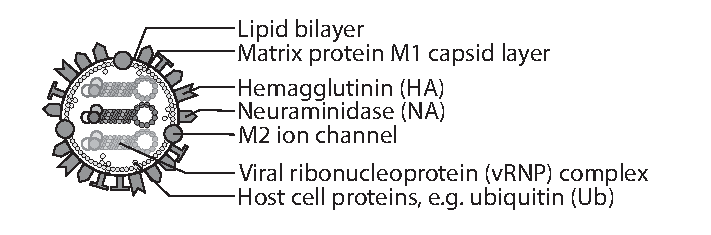
\includegraphics[width=0.95\textwidth, trim={0cm 0cm 0cm 0cm}, clip]{D_chapters/0_introduction/flu_structure.pdf}
\captionof{figure}{Influenza virus structure}
\label{figure:fluStructure}
\end{center}

The three largest vRNP segments - PB2, PB1, and PA - encode polymerase subunits responsible for viral RNA synthesis in the host cell nucleus.

Intermediate sized segments encode nucleoprotein (NP), which protects viral RNA strands, and two surface glycoprotein spikes HA and NA. The HA spike binds host cell-surface sialic acid receptors initiating viral entry. The NA spike cleaves sialic acid residues from the new viral particles to release them from the host cell.

Based on these glycoprotein spikes, influenza A viruses are categorized into antigenic subtypes. 18 HA and and 11 NA subtypes (named H1-18 and N1-11, respectively) have been identified so far \cite{InfluenzaAAntigenicSubtypes}. Thus, for example H3N2 virus contains a H3 subtype HA and a N2 subtype NA.

Segment M encodes the influenza matrix protein M1 which forms a protective capsid layer around vRNPs. Open reading frame shift during translation leads to production of ion channel protein M2, based on the same segment \cite{dubois2014influenza}.

Finally, the smallest segment NS encodes several non-structural proteins which assist the course of infection.

Influenza virus particles often carry host proteins, which they "borrow" from their host cell. Some of these host proteins, such as annexin A2, $\beta$-actin, and ubiquitin B are present in the virions in amounts exceeding native viral proteins NS1, M2, and NEP \cite{hutchinson2014conserved}. Currently, it is unclear whether these host proteins deliver any function during infection, or that their presence is simply an artifact of viruses hijacking cellular microvesicle formation pathways to produce enveloped virions \cite{hutchinson2014conserved}.